%!TEX root = master.tex

\section{Model-based Reinforcement learning}
This is a class of reinforcement learning algorithms that builds a model of the environments dynamics and reward structure to improve decision making, a policy. By approximating a model of the environment the model-based RL can plan better and faster. The model-based RL uses the model to simulate possible outcomes and optimize the actions accordingly. This approach can lead to more efficient learning, better exploration and improved generalization. Especially in environments with sparse rewards or limited data. 

\subsection{Repetition, if we do not have a model?}
We can use experience to estimate value functions: $S_t, A_t, R_{t+1}, S_{t+1}, A_{t+1}$ to make new estimates:

	\begin{equation}
		\text{New estimate} \leftarrow \text{Old estimate} + \text{Step size} [\text{Target} - \text{Old estimate}]
	\end{equation}

\begin{wbox}{Repetition}
\begin{itemize}
	\item \textbf{TD-Learning} to estimate $v_\pi(s,a)$
		\begin{equation}
			V(S_t) \leftarrow V(S_t) + \alpha [R_{t+1} + \gamma V(S_{t+1}) - V(S_t)]
		\end{equation}
	\item \textbf{SARSA} (on-policy): 
		\begin{equation}
			Q(S_t, A_t) \leftarrow Q(S_t,A_t) + \alpha[R_{t+1} + \gamma Q(S_t,A_t) - Q(S_t,A_t)] 
		\end{equation}
	\item \textbf{Q-learning} (off-policy):
		\begin{equation}
			Q(S_t, A_t) \leftarrow Q(S_t,A_t) + \alpha [R_{t+1} + \gamma \underset{a}{\text{max }}Q(S_t,A_t)]
		\end{equation}
		Possible alternative: Use the experience to estimate a model of the environment. 
\end{itemize}
\end{wbox}


\subsection{What is a model}
There are many ways to descrive what a model is, but here are two interesting quotes on the subject:


\begin{wbox}{}
\begin{center}
Anything we can use to answer questions about the environment without interacting
with it.” \\– \textbf{Lennart Ljung and Torkel Glad}

\vspace{0.5 cm}

“Essentially, all models are wrong, but some are useful.” \\– \textbf{George E. P. Box}
\end{center}
\end{wbox}

In reinforcement learning a \textbf{model} is something the \textbf{agent} can use to predict how the environment will respond to a given action. It can:
	
\begin{itemize}
	\item Produce a prediction of next state and reward: $(s,a) \rightarrow (\hat{s}^{\prime}, \hat{r}^{\prime}$
	\item Produce a prediction of next state $(s,a) \rightarrow \hat{s}^{\prime}$
\end{itemize}

A \textbf{distribution model} is a model that provides probabilities for all possible possibilities: $p(s^{\prime}, r|s,a)$. This is in general more difficult than the other type of model. \textbf{Sample model} provides us with one random sample from the possible outcomes. 

\subsection{Why model-based?}
The \textbf{advantages} with model-based RL is that the agent can learn a model with supervised learning that have more established methods. It has been used in classical control with success and for a wide range of different tasks. It is possible to use prior knowledge to reduce the number of unknown parameters. There is a similarity between model building and System identification in classical control. If feedback is used a perfect model is not typically not needed. With a model it is possible to reason about model uncertainty and offers more explainability. Transfer learning is an advantage were pre-existing knowledge and experience from one task is used to enhance performance in another related task. Examples of \textbf{disadvantages} with model-based RL are that estimated model might not capture the dynamics of the environment very well and the result may be a bad policy. By learning model and then construct the value function we have introduced two sources of approximation error. It is sometimes the case that the value function and optimal policy can be much simpler than an accurate model. 

\subsection{How to do model-based RL}
This can be done in many different ways but the most common methods are: 

\begin{enumerate}
	\item Learn a model of the environment (Supervised learning / System identification)
	\item Find the optimal policy for that model:
		\begin{itemize}
			\item Classical control  methods
			\item Dynamic programming 
			\item Q-learning, SARSA etc with the samples produced with the model
		\end{itemize}
\end{enumerate}

There are some possible extensions, for example to use some uncertainty measure and find a that is robust to this uncertainty. Here follows a list of examples models:

\begin{itemize}
	\item Table lookup
	\item Linear dynamic system 
	\item Gaussian process model
	\item Linear regression model
	\item Deep neural network
\end{itemize}


\subsection{Table lookup model}
The model is $p(s^{\prime},r|s,a)$ explicitly. Training data is collected $S_0, A_0, R_1, S_1, \ldots, R_T,A_T$ and used to estimate:

	\begin{equation}
		\hat{p} (s^{\prime},r|s,a) = \frac{1} {N(s,a)} \text{ (Number of times } (s^{\prime},r) \text{ came after } (s,a)) 
	\end{equation}

For a good model at $(s,a)$ we have to have seen this state-action pair many times. That is, exploration is still a very important part!

\subsection{Model-based and sample-based planning}
With a given estimated \textbf{model} $\hat{p}(s^{\prime},r|s,a)$ we can solve the MDP and use some of our favorite methods to do so: value iteration or policy iteration. With \textbf{sample-based} planning we use the model to generate samples for us. This a very simple but powerful approach. We then use sample experience from the model:

	\begin{equation}
	 	S_{t+1}, R_{t+1} \sim p(s^{\prime},r|S_t,A_t)
	 \end{equation} 
Then we apply \emph{model-free} RL to these model generated samples, with for example:

	\begin{itemize}
	 	\item Monte-Carlo control
	 	\item SARSA
	 	\item Q-learning
	 \end{itemize} 

 This can be very useful when sampling form the real world is very expensive. 

\subsection{Learning and planning}
In \emph{model-free} learning we don't have a model and must learn from real experience to train/learn our value functions. With \emph{Model-based} RL and \emph{sample-based} planning we learn a model from \textbf{real} experience and then learn the value function (and or policy) from the simulated experience. \emph{Dyna} or integrated learning and planning learns a model from experience and then learns the value function (and or policy) from \textbf{real} and \textbf{simulated} experience. 


\subsection{Dyna}
Dyna combines the model-based learning and direct learning from real experience. This enables the agent to learn and update its knowledge about the environment while at the same time improving its policy. The key concept is called \emph{experience replay} which allows the agent to learn from past experience and simulated experiences from the model which gives efficient exploration and decision making.

\begin{figure}[ht!]
\centering
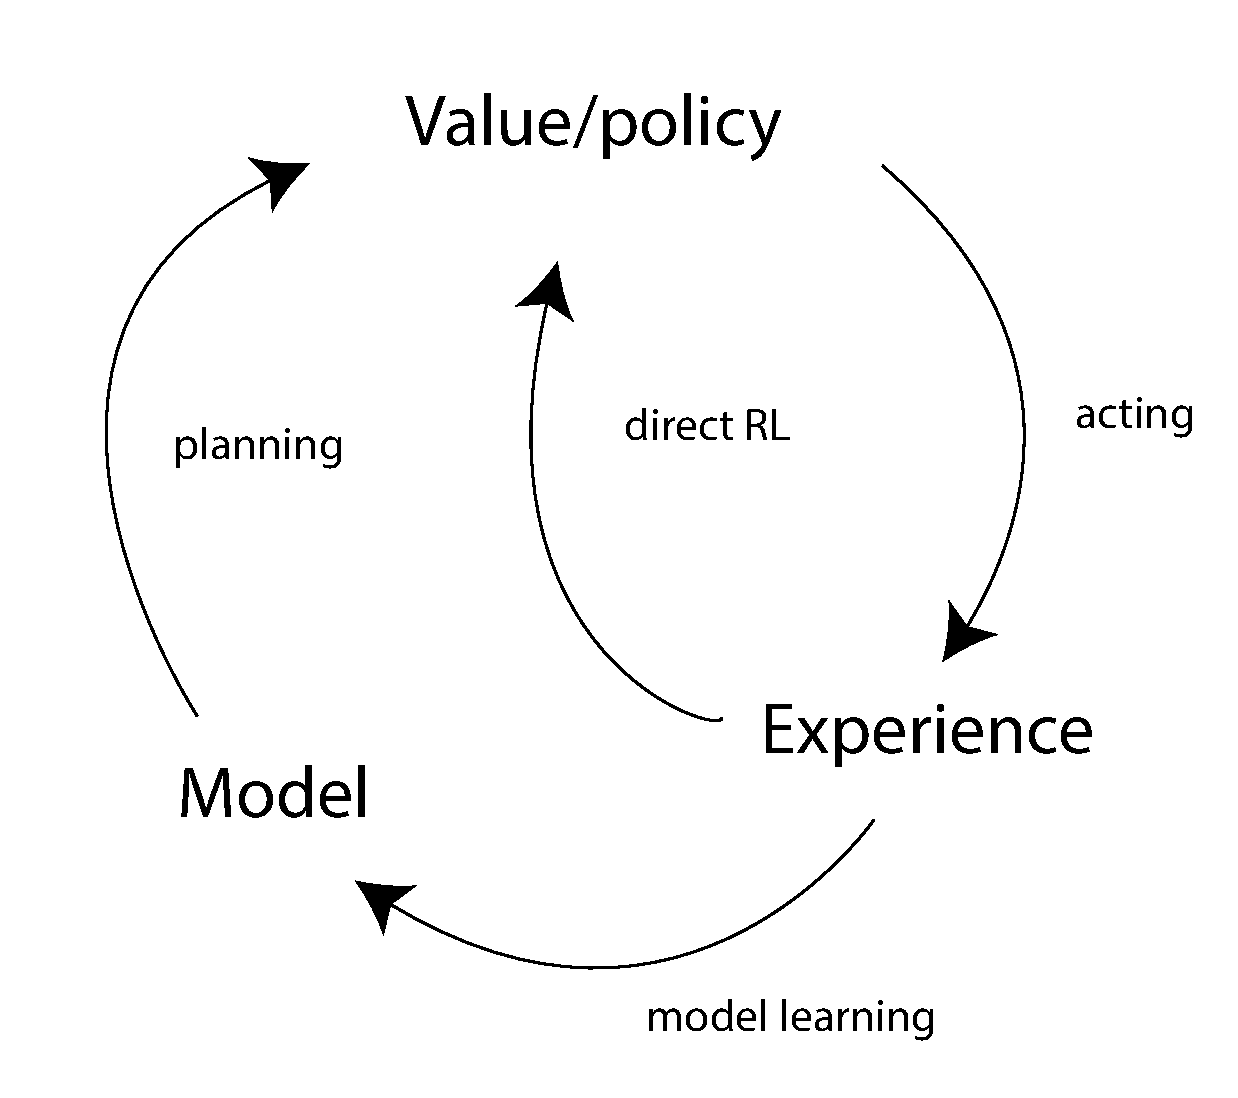
\includegraphics[width=80mm]{figures/dyna.pdf}
\caption{Dyna architecture}
\label{fig:dyna}
\end{figure}

 \subsection{Tabular Dyna-Q for deterministic environments}
 With model learning, if we observe: $S_t, A_t, R_{t+1}, S_{t+1}$ then :

 	\begin{equation}
 		\text{Model}(S_t,A_t) \leftarrow R_{t+1}, S_{t+1}
 	\end{equation}
 
And with Q-learning form both the simulated and real experience $S,A,R,S^{\prime}$ we can do:

	\begin{equation}
		Q(S,A) \leftarrow Q(S,A) + \alpha[R + \gamma \underset{a}{\text{max }} Q(S^{\prime},a)-Q(S,A)]
	\end{equation}

\begin{wbox}{Tabular Dyna-Q}
Initialize $Q(s,a)$ and Model$(s,a)$ for all $s \in \mathcal{S}$ and $a \in \mathcal{A(s)}$	 
Loop forever:
	\begin{enumerate}
		\item $S \leftarrow$ current (nonterminal) state
		\item $A \leftarrow \epsilon$-greedy$(S,Q)$
		\item Take action $A$; observe resultant reward $R$ and state $S^{\prime}$
		\item $Q(S,A) \leftarrow Q(S,A) + \alpha[R + \gamma \underset{a}{\text{max }} Q(S^{\prime},a)-Q(S,A)]$ 
		\item $\text{Model}(S_t,A_t) \leftarrow R_{t+1}, S_{t+1}$ (assuming that the environment is deterministic)
		\item Loop repeat $n$ times:
		\begin{itemize}
			\item $S \leftarrow$ random previously observed state
			\item $A \leftarrow$ random action previously taken in $S$
			\item $R,S^{\prime} \leftarrow $ Model$(S,A)$
			\item $Q(S,A) \leftarrow Q(S,A) + \alpha[R + \gamma \underset{a}{\text{max }} Q(S^{\prime},a)-Q(S,A)]$ 
		\end{itemize}
	\end{enumerate}
\end{wbox}


\subsection{DynaQ vs DynaQ+}
DynaQ is model biased, it (Naively) inherently assumes that the learned model is an accurate description of the real environment. So if the environment changes it takes time to adapt or in some cases it might take long time to discover a more efficient way to solve the task. DynaQ+ is a possible solution to this. The idea is to when simulating experience add a reward for exploring states not seen before: Specifically, if $R, S^{\prime} \leftarrow \text{Model}(S,A)$ then use:

	\begin{equation}
		R + \kappa \sqrt{\tau}
	\end{equation}

in the Q-update. Here $\tau$ is the number of time steps since $(S,A)$ was last visited in the real experience. We encourage the agent to visit states it has not seen for a long time. This extra exploration may cost some extra, but the curiosity can help if the real world changes for example.

\subsection{Exploration vs Exploitation trade-offs}
There is always a trade off in RL when it comes to exploration and exploitation. When we explore we gather more information and can find better policys but this cost us reward while we are doing this and there is always the possibility that we don't find a better policy either. With exploitation we make the best decisions from the knowledge we currently have and don't waste "energy" on trying to find better ways to do it. Some explorations ideas we seen so far are:

\begin{itemize}
	\item $\epsilon$-greedy
	\item  DynaQ+
	\item Optimistic initialization
\end{itemize}

\section{Model-based RL in continuous action and state spaces}
Now we will start talking about how we can extend the ideas that have been presented so far to continuous state and action spaces. In this case we can't store the Q-values for all possible state/action-pairs in a table any more and we will therefore use function approximations instead:

	\begin{equation}
	 	Q(s,a;\textbf{w}) \approx q_\pi(s,a)
	 \end{equation} 

There are many ways to do model-based RL in these situations. 

\subsection{A system identification approach}
If we assume that the dynamics of the environment can be accurately described as: 
	\begin{equation}
		s_{t+1} = f(s_t, a_t;\textbf{w})
	\end{equation}
where \textbf{w} is a vector of unknown parameter/weights. Here the $f(\cdot)$ can be a neural network, a basis expansion or a linear system. Data/experience is to be collected ($S_0,A_0,S_1,\ldots,A_{t-a},S_T$), learning the model using the prediction error method:

	\begin{equation}
		\hat{\textbf{w}} = \underset{w}{\arg \text{max }}\sum_{t=0}^{T-1} ||S_{t+1} - f(S_t,A_t;\textbf{w})||^{2}_2
	\end{equation}

Finding a policy can be done using \emph{classic control} or \emph{model-free} RL using the samples from the model.














